% mnras_template.tex 
%
% LaTeX template for creating an MNRAS paper
%
% v3.0 released 14 May 2015
% (version numbers match those of mnras.cls)
%
% Copyright (C) Royal Astronomical Society 2015
% Authors:
% Keith T. Smith (Royal Astronomical Society)

%%%%%%%%%%%%%%%%%%%%%%%%%%%%%%%%%%%%%%%%%%%%%%%%%%
\documentclass[fleqn,usenatbib]{mnras}
% MNRAS is set in Times font. If you don't have this installed (most LaTeX
% installations will be fine) or prefer the old Computer Modern fonts, comment
% out the following line

\usepackage{newtxtext,newtxmath}
% Use vector fonts, so it zooms properly in on-screen viewing software
% Don't change these lines unless you know what you are doing
\usepackage[T1]{fontenc}

% Allow "Thomas van Noord" and "Simon de Laguarde" and alike to be sorted by
% "N" and "L" etc. in the bibliography.  Write the name in the bibliography as
% "\VAN{Noord}{Van}{van} Noord, Thomas"
\DeclareRobustCommand{\VAN}[3]{#2}
\let\VANthebibliography\thebibliography
\def\thebibliography{\DeclareRobustCommand{\VAN}[3]{##3}\VANthebibliography}

%%%%% AUTHORS - PLACE YOUR OWN PACKAGES HERE %%%%%
\usepackage{graphicx}
% \usepackage{amsmath}
% \usepackage{amssymb}
\usepackage{cuted}
\setlength{\stripsep}{0ex}

\usepackage{tcolorbox}
\usepackage{listings}

%%%%%%%%%%%% CUSTOM COMMANDS %%%%%%%%%%%%%%%%%%%%%

\newcommand{\citneeded}{{\bf \color{red} $^{\text{citation needed}}$}}
\newcommand{\todo}[1]{{\bf \color{red} #1}}
\newcommand{\notes}[1]{{\color{cyan} #1}}

\newcommand{\Gradus}{Gradus.jl }
\newcommand{\relline}{\texttt{relline} }

\newcommand{\e}{\text{e}}
\renewcommand{\d}{\text{d}}
\newcommand{\rg}{r_\text{g}}
\newcommand{\utensor}[3]{#1^{#2}_{\phantom{#2}#3}}
\newcommand{\dtensor}[3]{#1_{#2}^{\phantom{#2}#3}}
\newcommand{\stensor}[3]{#1_{#2}^{#3}}
\newcommand{\deriv}[2]{\frac{\d #1}{\d #2}}
\newcommand{\pderiv}[2]{\frac{\partial #1}{\partial #2}}
\newcommand{\risco}{r_\text{ISCO}}

\newcommand{\vel}[1]{v^{#1}}
\renewcommand{\vector}[1]{\mathbf{#1}}
\newcommand{\jacobian}[2]{\left\lvert \frac{\partial #1}{\partial #2} \right\rvert}

\renewcommand{\Im}[1]{\text{Im}\left[#1\right]}
\renewcommand{\Re}[1]{\text{Re}\left[#1\right]}

%%%%%%%%%%%%%%%%%%% TITLE PAGE %%%%%%%%%%%%%%%%%%%

\title[Gradus.jl]{Gradus.jl: general relativistic ray-tracing and reverberation modelling through automatic differentiation}
\author[F. J. E. Baker et al.]{
F. J. E. Baker,$^{1}$\thanks{E-mail: fergus.baker@bristol.ac.uk (FB)}
and A. J. Young$^{1}$
\\
$^{1}$H. H. Wills Physics Laboratory, Tyndall Avenue, Bristol BS8 1TL, UK
}
% These dates will be filled out by the publisher
\date{Accepted XXX. Received YYY; in original form ZZZ}
% Enter the current year, for the copyright statements etc.
\pubyear{2023}

% Don't change these lines
\begin{document}
\label{firstpage}
\pagerange{\pageref{firstpage}--\pageref{lastpage}}
\maketitle
% Abstract of the paper
\begin{abstract}
	We introduce \Gradus, an open-source...
\end{abstract}

% Select between one and six entries from the list of approved keywords.
% Don't make up new ones.
\begin{keywords}
keyword1 -- keyword2 -- keyword3
\end{keywords}

%%%%%%%%%%%%%%%%%%%%%%%%%%%%%%%%%%%%%%%%%%%%%%%%%%

%%%%%%%%%%%%%%%%% BODY OF PAPER %%%%%%%%%%%%%%%%%%

%%% INTRODUCTION %%%%%%%%%%%%%%%%%%%%%%%%%%%%%%%%%
\section{Introduction}

\notes{
In the era of quantitative, precision observational tests of General Relativity in the strong field regime it is necessary to have a fast and flexible method to compute the observational properties of accreting black hole systems. We have developed an open-source integrator 
\Gradus\footnote{Open-source and available under MIT license at \url{https://github.com/astro-group-bristol/Gradus.jl}.} for this purpose. In the remainder of the paper we describe how the software works, comparing with previous work in the literature, and outlining the new capabilities of \Gradus.

% Maybe some history of the problem with key references
Transfer functions \citep{cunningham_effects_1975} % An example reference

Julia is a high-performance... with SciML and DifferentialEquations.jl, a state-of-the-art ecosystem and workhorse for solving differential equations. 
}

\todo{goerge and fabian for reflection of xrays off cold ad}

\subsection{A short review of general relativistic ray tracing}

\todo{
\begin{itemize}
    \item review other softwares
    \item where does Gradus fit into the field (extensibility / maintainability / prototyping models)
    \item define SSD as Shakura Sunyaev disc
\end{itemize}
}

The trajectory of light in curved space may be determined by reformulating the
Hamilton-Jacobi equations of motion as a first-order ordinary differential
equation (ODE) system. 

A second-order ODE system may alternatively be formulated directly from the
geodesic equation; a method which is pedagogically simpler, but computationally
more expensive than the first-order system, as either the full metric
connection or derivatives of the metric must be explicitly implemented, else
approximated at cost during runtime. With advancements in automatic
differentiation, derivatives are cheap to compute, and consequently the
second-order approach is tractable and both a parsimonious and spacetime
agnostic method for computing geodesics.

%%% NUMERICAL METHODS %%%%%%%%%%%%%%%%%%%%%%%%%%%%
\section{Numerical methods}

For simplicity, we focus on static, axisymmetric spacetimes in the
Boyer-Lindquist coordinates. Such spacetimes have metrics of the form 
\begin{equation}
\label{eq:static_axisymmetric_metric}
    g_{\mu\nu} 
    = g_{tt} \d t^2 
    + g_{rr} \d r^2 
    + g_{\theta\theta} \d \theta^2 
    + g_{\phi\phi} \d \phi^2 
    + 2g_{t\phi} \d t \d \phi.
\end{equation}
We adopt $(-, +, +, +)$ metric signature and standard units $c = G = 1$. Greek
indices ($\mu, \nu$) denote the four spacetime components, and Latin indices
($i, j$) the three spatial components. We write partial derivatives with
respect to the coordinates $x^\mu$ as $\partial_\mu := \partial / \partial
x^\mu$.

We integrate the differential equation systems principally with the adaptive
Tsitouras Runge-Kutta pairs of order 5/4 \citep{tsitouras_rungekutta_2011}.
This integrator is known to be fast and robust, and provides `free'
fourth-order interpolants of the resulting solutions. We use the interpolation
when additional quantities need to be re-calculated along a given trajectory,
for accurately calculating points of intersections, and for visualization
purposes, as will be discussed throughout this section.

\subsection{Geodesic integration}

Using coordinates $x^\mu$, the geodesic equation with instantaneous external
acceleration $a^\mu$ is written
\begin{equation}
\label{eq:geodesic_equation}
    \frac{\d^2 x^\mu}{\d \lambda^2}
    + \utensor{\Gamma}{\mu}{\nu\sigma}
    \vel{\nu}
    \vel{\sigma}
    = a^\mu,
\end{equation}
where $\lambda$ is the affine parameter and $v^\mu = \d x^\mu / \d \lambda$ is
the four-velocity. The effects of spacetime curvature on the trajectory are
encoded in the Christoffel connections, 
\begin{equation}
\label{eq:christoffel}
    \utensor{\Gamma}{\mu}{\nu\sigma}
    := \frac{1}{2} g^{\mu\rho} 
    \left(
        \partial_{\nu}g_{\rho \sigma}
        + \partial_{\sigma}g_{\rho \nu}
        - \partial_{\rho}g_{\sigma \nu}
    \right).
\end{equation}
For a given metric, the geodesic equation is a set of four coupled second order
differential equations that can be solved with a choice of initial $x^\mu$ and
$\vel{\mu}$. We are free to to choose an initial position with $x^t = 0$, and
are forced to constrain the velocity by the invariance
\begin{equation}
\label{eq:velocity_constraint}
    g_{\sigma\nu} \vel{\sigma} \vel{\nu} = \mu^2,
\end{equation}
where $\mu$ is the invariant mass. This constraint gives rise to three solution
classes depending on the sign of $\mu^2$, namely $\mu^2 = 0$ corresponding to
null-, $\mu^2 > 0$ to time-, and $\mu^2 < 0$ to space-like geodesics. Null
geodesics are the trajectories of photons, time-like geodesics are the
trajectories of massive particles, and space-like geodesics are the
trajectories of exotic particles, such as tachyons \citneeded. 

Derivatives of the metric needed in Eq. \eqref{eq:christoffel} are efficiently
computed with AD. This brings versatility, as new spacetimes need only define
the metric for the geodesic ODE system to be solvable. If the class of
spacetime exhibits additional symmetries, these can be exploited to reduce
computation further: for example, metrics of the form
\eqref{eq:static_axisymmetric_metric} exploit $\partial_t g_{\mu\nu} =
\partial{\phi} g_{\mu\nu} = 0$ and avoid calculating two columns of the
Jacobian entirely.

It is sufficient to specify the three-vector $\vel{i}$ to determine $\vel{t}$
by rearranging Eq. \eqref{eq:velocity_constraint} as
\begin{equation}
\vel{t}  = \frac{-g_{t\phi} \vel{\phi} \pm
    \sqrt{-g_{ij} \vel{i} \vel{j} - \mu^2}
}{g_{tt}}.
\end{equation}
The choice of positive or negative root corresponds to the direction of time,
wherein lies the ray-tracing \textit{trick}: a time-reversal symmetry in the
metric allows us to trace from an observer back to the point of origin, and
then \textit{reverse} time in order to calculate quantities as seen by the
observer. \todo{explain better}

\subsection{Observers and emitters}

\begin{figure}
    \centering
    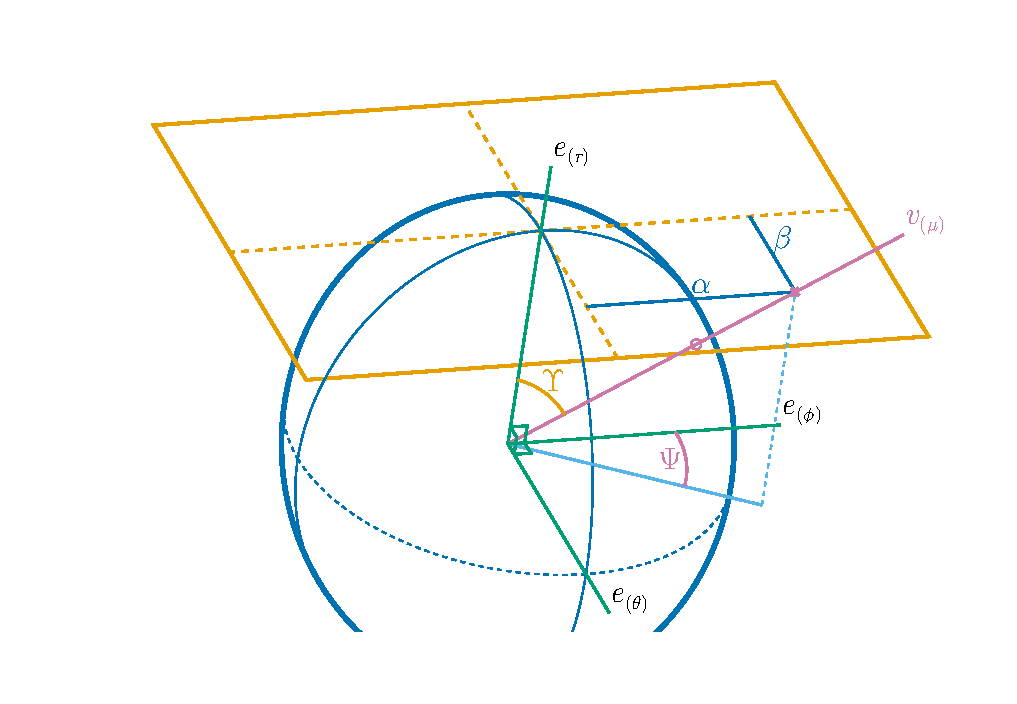
\includegraphics[width=0.99\linewidth]{figures/skycoords.pdf}
    \caption{
    Geometry of the local sky for an observer or emitter. The image plane is
    perpendicular to the $e_{(r)}$ axis, which for an observer points towards
    the global origin and therefore the central singularity. The momenta
    $v_{(\phi)}$ and $v_{(\theta)}$ are used to calculate the impact parameters
    on the image plane, $\alpha$ and $\beta$ respectively. For emitters, the
    angles $(\Upsilon, \Psi)$ are used to parameterize points on the local sky,
    that may be decomposed onto the basis $e_{(i)}$ to find $v_{(\mu)}$.
    }
    \label{fig:observer-coordinates}
\end{figure}

We calculate the initial velocity vector differently depending on whether we are
considering an observer or an emitter. For observers, we are interested in the
sparse set of emitted photons which reach an image plane representing the
observer's field of view, and therefore parameterize the velocity vector using
\emph{impact parameters} on the image plane. The parameters representing the
local sky of an observer is shown in Fig.~\ref{fig:observer-coordinates}.
Following \cite{cunningham_optical_1973}, one may then define a set of impact
parameters from components of the local momenta
\begin{align}
    \alpha &:=  x^r \frac{v_{(\phi)}}{v_{(r)}}, \\
    \beta &:= x^r \frac{v_{(\theta)}}{v_{(r)}},
\end{align}
using indices in parentheses to denote the vector components in the local
frame. The choice of subscript ($r, \theta, \phi$) is to anticipate an
identification between local and global bases, and to provide some intuition
for the local frame.

Exploiting the invariance of four-momenta (c.f. Eq.
\eqref{eq:velocity_constraint}), we obtain a curve of solutions for the local
momenta of geodesics intersecting the image plane at specific $\alpha$ and
$\beta$
\begin{align}
    \frac{v_{(r)}}{v_{(t)}} &= -\left( \sqrt{1 + \left(\frac{\alpha}{x^r}\right)^2 + \left(\frac{\beta}{x^r}\right)^2} \right)^{-1} = \mathscr{R}, \\
    \frac{v_{(\theta)}}{v_{(t)}} &= \mathscr{R} \frac{\beta}{x^r}, \\
    \frac{v_{(\phi)}}{v_{(t)}} &= \mathscr{R} \frac{\alpha}{x^r}.
\end{align}

The case for emitters is subtly different, where expressions for these momenta
components are obtained by considering the direction of emission on the local
sky. That is, by projecting an initial velocity tangent vector pointing in the
direction of the angles $(\Upsilon, \Psi)$ onto the local momentum frame.  This
is compactly written with an intermediary decomposition onto a Cartesian
coordinate system as
\begin{equation}
    \label{eq:local-angle-to-velocity}
    \frac{v_{(i)}}{v_{(t)}} = \frac{1}{v_{(t)}}
    \left[\pderiv{(x, y, z)}{(r, \theta, \phi)}\right]
    \left(
    \begin{matrix}
        \sin \Upsilon \cos \Psi \\
        \sin \Upsilon \sin \Psi \\
        \cos \Upsilon \\
    \end{matrix}
    \right),
\end{equation}
where the partial derivative term denotes the cartesian to spherical coordinate
Jacobian. The component $v_{(t)}$ is the negative of the energy in the local
frame, and is conventionally set to $-v_{(t)}=E=1$ without loss of generality. 

For both observers and emitters, we must identify a local frame, where the
natural choice is the locally non-rotating frame (LNRF)
\citep{bardeen_rotating_1972} \todo{check citation + explain significance}. The
transformation from local to global coordinates is
\begin{equation}
    \label{eq:local-to-global-velocity}
    v_\mu = \e^{(\nu)}_{\phantom{(\nu)}\mu}\  v_{(\nu)}
\end{equation}
where the basis vectors $\e^{(\nu)}_{\phantom{(\nu)}\mu}$ (or tetrad) are found
using the theorem of Gram-Schmidt (\citealp{schmidt_uber_1989}, Appendix
\ref{appendix:gram-schmidt}). The formalism may be extended for an observer or
emitter in motion, where their velocity modifies the mapping by a local Lorenz
transformation, $\Lambda^{(\kappa)}_{\phantom{(\kappa)}(\nu)}$, as 
\begin{equation}
    v_\mu = \e^{(\nu)}_{\phantom{(\nu)}\mu}\  \Lambda^{(\kappa)}_{\phantom{(a)}(\nu)} v_{(\kappa)}.
\end{equation}
This Lorenz transformation may be absorbed into the tetrad with careful
construction, using the velocity of the observer or emitter as
$\utensor{\e}{(t)}{\mu}$, and orthogonalizing using the theorem of Gram-Schmidt.

As a note, the impact parameters are calculated from the constants of motion in
\cite{cunningham_optical_1973}, with the assumption that the observer is
situated in asymptotically flat space, whereas our calculations are specific to
the location of the observer in the spacetime. We approximate asymptotically
flat space by positioning our observer at radial distance $r_\text{obs} > 10^4
\rg$, however codes that make use of the results in
\cite{cunningham_optical_1973} will suffer an error of order
$\sim1/r_\text{obs}$ due to the assumed asymptotic energy and local energy at
that distance differing. This must be taken into account when comparing codes.

\subsection{Special orbits and horizons}
\label{sec:special-orbits}

Of particular interest when studying accreting processes are the Keplerian
circular orbits, confined to the equatorial plane f$(x^\theta = \pi/2)$ in
axis-symmetric spacetimes. A subset of the Keplerian orbits are the circular
orbits, and are therefore relevant in analytical models of accretion discs
\citep{shakura_black_1973}. These circular orbits are stationary points of the
geodesic Hamiltonian, and constrained by $v^r = v^\theta = 0$.  These orbits are
often studied analytically, and have a general solution for metrics of the form
\citep{eq:static_axisymmetric_metric} (e.g. \citealp{johannsen_regular_2013},
We provide a derivation with some extension towards $a^\mu \neq 0$ in Appendix
\ref{appendix:circular-orbits}).

Circular orbits are classified as either stable or unstable
\citep{wilkins_bound_1972,bardeen_rotating_1972}. There exists an innermost
stable circular orbit radius (ISCO, denoted $\risco$), below which orbits
are energetically hyperbolic: small perturbations will send test particles
escaping to infinity or spiralling into the central singularity. The stability of
an orbit depends on the sign of $\d E / \d x^r$, with $>0$ corresponding to
energetically stable configurations. The ISCO is the critical point at
which 
\begin{equation}
    \label{eq:isco-definition}
    0 = \left. \frac{\d E}{\d x^r} \right\rvert_{x^r := \risco}.
\end{equation}
Stable circular orbits are only possible for radii $x^r \geq \risco$.
Within the ISCO is the so-called \textit{plunging region} where $v^r \neq 0$.
\citneeded

Stable orbits may also be determined purely from the numerical integration of
geodesics, by mandating a stability measure and optimizing the initial velocity
vector until some heuristic measure is a minimum. For example, let $\mathscr{M}$
measure the eccentricity of an orbit in the equatorial plane. For a given radius
$x^r$, the velocity corresponding to a circular orbit is $v^\mu = v^t \partial_t
+ v^\phi \partial_\phi $. With \eqref{eq:velocity_constraint}, the circular
orbit velocity may be found through
\begin{equation}
    \underset{v^\phi}{\arg \min}\ \ \mathscr{M}(x^r, v^\phi),
\end{equation}
using a numerical optimizer. We use the Nelder-Mead simplex method as our
preferred optimization algorithm for exploring the $v^\phi$ parameter space
\citep{nelder_simplex_1965}. Due to only integrating finite windings of the
orbit, this approach may find both unstable and stable orbits. These are 
distinguished by inspecting $E$ as a function of $x^r$, or similarly $E$ as a
function of $L_z$ \citep{hackmann_charged_2013}, see Figure \ref{fig:e-lz-cusp}.
The $\risco$ is found by solving \eqref{eq:isco-definition} numerically, or
by finding $x^r$ corresponding to the \emph{cusp} of the curve of  $E$ against
$L_z$.

\begin{figure}
    \centering
    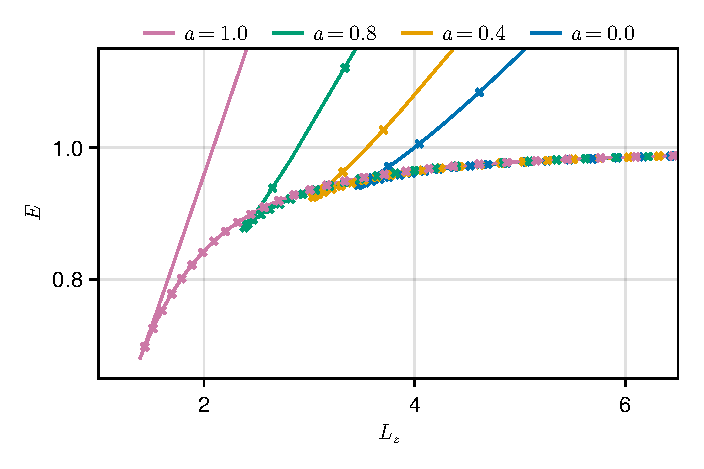
\includegraphics[width=0.95\linewidth]{figures/circular-orbits.E-Lz.pdf}
    \caption{\todo{TODO, also show the points we calculate using the numeric orbit finder}}
    \label{fig:e-lz-cusp}
\end{figure}

The velocities of orbits in the plunging region are numerically calculated by
``dropping'' a test particle from $\risco -  \delta x^r$, and tracing for a
large interval of proper time, until the fate of the geodesic is realized. The
components of $v^\mu$ are then interpolated over $x^r$ to approximate analytic
solutions. Figure \ref{fig:circular-orbit-error} illustrates the accuracy of our
numerical method for determining such plunging orbits.

This heuristic optimization technique is also used for other objective
functions, such as for solving for the initial conditions of  geodesics that
intersect a chosen point in the spacetime ($\mathscr{M}$ measures closest
approach), or that exhibit some specific desired features (e.g. $\mathscr{M}$
measures periodicity).

We implement a numerical method for determining the event horizon radius using a
similar approach.

\todo{The following are stubs that need expanding}
The Keplerian orbits exhibit a number of other interesting radii that may be
calculated from the energy of the orbit. 

The photon orbit is the radius for which $E / \mu = \infty$, which is the only
radius for which null geodesic orbits are circular. 

At $E / \mu = 1$ is the so-called \emph{marginally bound} orbit.

Similar techniques used to calculate the radii special orbits are used to
determine the event horizon radius. Under axis-symmetry, the event horizon is
the set of the $(r, \theta)$ coordinates that satisfy
\begin{equation}
    \todo{equation}
\end{equation}
For a set of equally spaced $\theta$, we determine $r$ by solving for the roots
of the equation using the Roots.jl package\citneeded .

\subsection{Charts and horizons}

A chart is used to terminate geodesic integration to avoid continuing
computation when the fate of a given geodesic is determined. In practical terms,
the chart is defined by a set of boundaries, and used to classify the outcome of
an integration. As a motivating example, consider a chart with an inner and
outer boundary: the inner boundary is a coordinate singularity of the metric,
$r_s$ (i.e. an event horizon), whereas the outer boundary is treated as the
\textit{effective infinity}, $r_\infty$. Geodesics at the inner boundary are
classified as lost behind the coordinate singularity, whereas those that reach
the outer boundary are considered to escape to infinity with no further
deviation to their trajectory. Additional boundaries of the chart may be used to
represent accretion geometry: by terminating the integration when the geodesic
crosses such a boundary, we consider the geodesic to have intersected the
surface of the accretion disc. 

The event horizon radius, $r_s$, used as the default inner boundary, may be
calculated for a metric of the form \eqref{eq:static_axisymmetric_metric} by
solving
\begin{equation}
    \label{eq:event_horizon}
    0 = \left. \frac{1}{g_{rr}} \right\rvert_{x^r = r_s}.
\end{equation}
For axisymmetric metrics, $g_{rr}$ may be a function of both $x^r$ and
$x^\theta$, in which case the inner boundary of the chart is a function of the
poloidal coordinate. If no analytic function for $r_s$ is known, it may be
numerically approximated using root solving methods.

In practice, close to the inner radius the adaptive time step of an ODE
integrator tends to shrink dramatically due to near-singular derivatives,
causing the integration to slow to almost a standstill. This may be avoided by
scaling the inner horizon with the choice of constant $\mathcal{K} > 0$, such
that $\tilde{r}_s = (1 + \mathcal{K}) r_s$, terminating the integration early
when $x^r \leq \tilde{r}_s$. This constant may be adjusted depending on how
vital it is for a geodesic to be able to glance the event horizon. We have
chosen $\mathcal{K} = 10^{-2}$ by default, as it dramatically improves
integration time without impacting the majority of simulations. 

Chart intersection is found using either an interpolating root-solver with
\texttt{ContinuousCallback} or a per-point test with \texttt{DiscreteCallback}
from DifferentialEquations.jl \citep{}.


\subsection{Computing observables}
\label{sec:computing-observables}

We consider \textit{observables} to be any physical quantity calculated from a simulation that is evaluated using some or all of the points along a geodesic. Often only the start and end point of a geodesic are required to calculate some physical quantity, and under such circumstances it is computational beneficial to avoid allocating space for the full solutions.

A frequently required quantity is the redshift along a geodesic, due to both the Doppler and gravitational redshift. This is compactly written as the ratio of energies between the start and end point connected by the geodesic,
\begin{equation}
\label{eq:redshift}
g := \frac{E_\text{end}}{E_\text{start}} = \frac{\left. v_\mu u^\mu \right\rvert_\text{end}}{\left. v_\mu u^\mu \right\rvert_{\text{start}}},
\end{equation}
where $v_\mu$ are the photon momenta, and $u^\mu$ the velocity of the emitting (start) and observing (end) media respectively.

Observables that require multiple points along the geodesic to be determined may either be calculated coincidentally with the geodesic equation, or subsequently re-traced along the ray. Such quantities include polarization / parallel transport or radiative transfer / optical depth. Calculating the quantities simultaneously has the benefit that the error tolerance in the step size estimation of the integrator is sensitive to changes in the observable. The benefit of the latter is that for a given set of metric parameters and observer inclination, the geodesics trajectories are unchanged, allowing the observable to be more efficiently recalculated with new parameters.


\subsection{Emissivity profiles}
\label{sec:emissivity-profiles}

The emissivity profile is the illumination pattern on an accretion disc, with the emissivity $\varepsilon$ being proportional to the illuminating flux absorbed per unit area \citep{laor_line_1991,wilkins_understanding_2012}. The source of illumination is thought to be a luminous corona with a given emission spectrum and morphology. The corona is often assumed to be a point source on the spin axis of the black hole, and that the illuminating flux on the disc is therefore axis symmetric \citep{fukumura_accretion_2007}, though extended sources are possible \citep{gonzalez_probing_2017}. \todo{there must be another reference here?} For these point sources, the emissivity profile is a function of the radial coordinate on the disc. The flux is approximated as the number of geodesics striking an annulus of the disc, along with some intensity function representing the emission spectrum of the corona, such that 
\begin{equation}
    \varepsilon (r, \d r) = \frac{\mathcal{N}(r, \d r)}{\gamma \tilde{A}(r, \d r)} I(g),
\end{equation}
where $\mathcal{N}$ is the geodesic count in an annulus $r + \d r$, $I$ is the intensity of the illuminating flux as a function of redshift $g$, $\tilde{A}$ is the relativistically corrected (proper) area of the annulus due to spacetime curvature, and $\gamma$ is the Lorentz factor that accounts for area contraction of the annulus due to the velocity of the disc. The orbital profile of the disc is assumed to follow Keplerian circular orbits in the equatorial plane.

The corrections are calculated as follows: for an infinitesimal area $\d A = \d r \d\phi$, the \textit{proper area} is calculated directly from the metric,
\begin{equation}
    \d\tilde{A} = \sqrt{g_{rr} g_{\phi\phi}}\, \d r\, \d \phi,
\end{equation}
which is the area as measured by a stationary observer in the disc, whereas the relativistic Lorentz factor is calculated as
\begin{equation}
    \gamma = \frac{1}{\sqrt{1 - \left(v^{(i)}\right)^2}},
\end{equation}
where $v^{(i)}$ are the spatial components of the angular velocity in the LNRF. These components are calculated with the tetrad basis as
\begin{equation}
    v^{(i)} = \frac{\utensor{\e}{(i)}{\mu}\, v^\mu}{\utensor{\e}{(t)}{\sigma}\, v^\sigma},
\end{equation}
where the special case of circular orbits only has $v^{(\phi)}$ non-zero.

The intensity function for the illuminating corona is usually assumed to be a powerlaw $I(g) = g^{-\Gamma}$ with varying photon index $\Gamma$ \citep{gonzalez_probing_2017}.

The emission from the corona is assumed to be locally isotropic in the rest frame of the corona. This is numerically determined by sampling $(\Upsilon, \Phi)$ evenly on a sphere, and transforming via \eqref{eq:local-angle-to-velocity} and \eqref{eq:local-to-global-velocity} to find the initial velocity of the geodesic. Those geodesics that intersect with the disc are then used to calculate the emissivity.

An alternative method for calculating the flux from point sources is detailed in \cite{dauser_irradiation_2013}, where the axis-symmetry is further exploited. This method determines the radii of the annuli by tracing photons that are emitted at equally spaced angles $\Delta \Upsilon$ in the source frame, and using the radial coordinate of geodesics where they intersect the disc $\Delta r$ as a proxy for the reciprocal number density. Since in three spatial dimensions, the poloidal coordinate must be distributed as a $\sin \Upsilon$ distribution for isotropic emission, $\varepsilon$ is weighted similarly\footnote{Instead of equally spaced $\Upsilon$, one may instead sample $\Upsilon \sim \cos (1 - 2 \mathcal{U})$, where $\mathcal{U}$ is a uniform distribution $\mathcal{U}(0,1)$. In this case, there is no $\sin \Upsilon$ weight in $\varepsilon$. This result may be shown using the inverse-CDF or Smirnov transform method.}
\begin{equation}
    \varepsilon(r, \Delta r) = \frac{\sin \Upsilon}{\gamma \tilde{A}(r, \Delta r)} I(g).
\end{equation}
The differences between these two methods is shown in Figure \ref{fig:coronal-tracing}. It should be noted that the latter method converges faster than the (Monte-Carlo) sampling of $\mathcal{N}$, and captures the behaviour at small $r$ close to the ISCO faithfully. However, since this method is specialized for point sources, extended corona require an approximate rebinning algorithm to reconstruct the emissivity profile taking into account the overlap between the annuli determined from different source points.

\begin{figure}
    \centering
    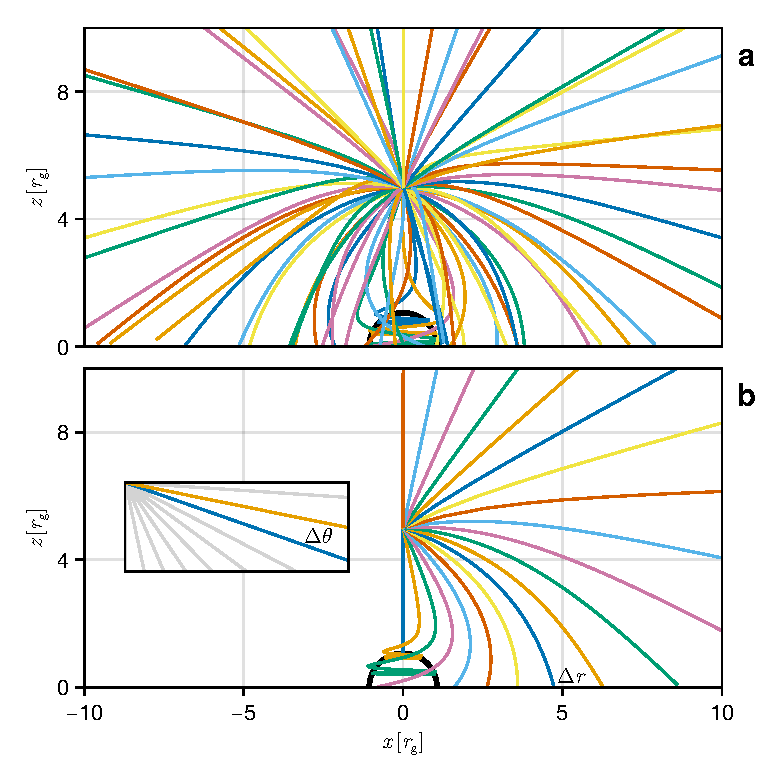
\includegraphics[width=0.95\linewidth]{figures/emissivity.coronal-traces.pdf}
    \caption{\todo{caption}}
    \label{fig:coronal-tracing}
\end{figure}

When axis-symmetry does not apply, we have developed a method for calculating the emissivity field as a function of $(r, \phi)$ on the disc. Here the points of intersection on the disc become the generators of a Delauney tesselation, such that the (relativistically corrected) Voronoi area may be used as a proxy for $\mathcal{N} /\tilde{A}$ (see Appendix \ref{appendix:voronoi}) in the limit of high sample count.

\subsection{Transfer functions}
\label{sec:transfer-functions}

\begin{figure*}
    \centering
    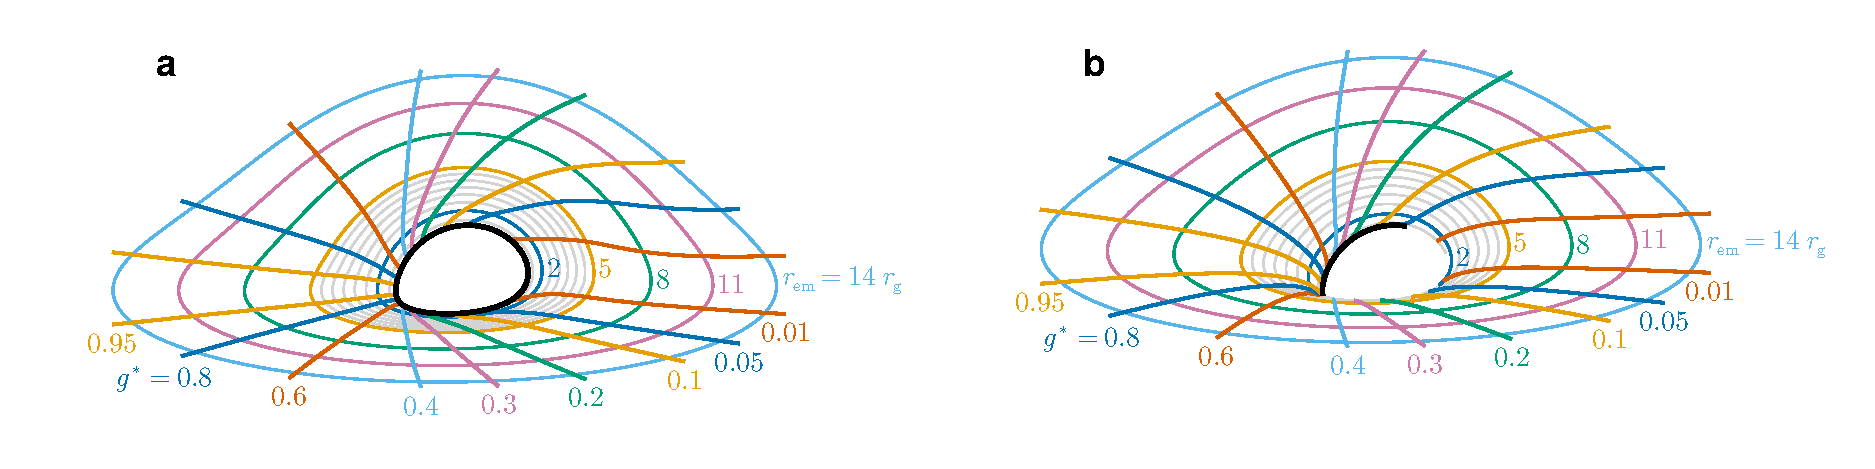
\includegraphics[width=0.95\linewidth]{figures/transfer-function.parameterization.pdf}
    \caption{Concentric rings of radius $r_\text{em}$ and contours of constant dimensionless redshift $g^\ast$ on disc in the equatorial plane, projected on the image plane of a distant observer at $\theta_\text{obs} = 75^\circ$. The central singularity is described by the Kerr metric with $a = 0.998$. The innermost thick black line is the projection of the ISCO. Note the contours of $g^\ast$ are double valued for any given $r_\text{em}$. Panel a) geometrically thin disc. Panel b) SSD with $\dot{M} / \dot{M}_\text{Edd} = 0.3$, with obscuration of some of the inner radii. The edge of the ISCO is here only partially visible.}
    \label{fig:transfer-parameterisation}
\end{figure*}

A particular observable that is frequently calculated with GRRT is the flux coming from a particular model of an accreting black hole. The infinitesimal flux is
\begin{equation}
\label{eq:infinitesimal-flux}
\d F(E, t) = I\left(E, t\right)\, \d \Omega,
\end{equation}
for observed energy $E$, time $t$, intensity $I$ and solid angle $\d \Omega$ on the observer's sky.

Using Liouville's theorem -- that the number density of photons in phase space is conserved -- the observed and emitted intensities are related by
\begin{equation}
\label{eq:liouville-theorem}
    I\left( E, t \right) = g^3 I_\text{em}\left(E_\text{em}, t_\text{em}\right).
\end{equation}
\todo{is this $t_\text{em}$ or just $t$??}
Integrating over $\d \Omega$ is equivalent to integrating over the image plane $\d \alpha \d \beta$, which in practical terms is binning the geodesic in each pixel by $E$ and $t$. In this formulation, for any change in $I_\text{em}$, the geodesic calculation would have to be recomputed, or a large table of values related to each geodesic stored, to finite precision. The sampling over the image plane similarly plays an important role, especially in increasing efficiency, since most of the variation in $I_\text{em}$ is sourced close to the ISCO, which can be under-resolved on coarse image planes. This may lead to oversampling regions of low or zero variation further out on the disc.

To elide this problems, and to be able to succinctly cache geodesic computation, the relativistic effects are often encoded in so-called \emph{transfer functions}, first introduced in \cite{cunningham_effects_1975},
\begin{equation}
    f:=\frac{g}{\pi r_\text{em}} \sqrt{g^\ast(1 - g^\ast)} \jacobian{(\alpha, \beta)}{(r_\text{em}, g^\ast)},
\end{equation}
where $r_\text{em}$ is the emission radius on the disc, and
\begin{equation}
    g^\ast := \frac{g - g_\text{min}}{g_\text{max} - g_\text{min}} \in [0, 1],
\end{equation}
is a rescaled dimensionless redshift parameter, and the extremal $g$ is calculated over a given $r_\text{em}$. This $g^\ast$ parameterization is double-valued everywhere except at $g^\ast = 0$ and $g^\ast = 1$, illustrated in Figure \ref{fig:transfer-parameterisation}. The transfer functions $f$ are then ostensibly a change-of-variable Jacobian, re-parameterizing the projected image of the disc from $(\alpha, \beta)$ to $(r_\text{em}, g^\ast)$. The additional elliptical envelope in $g$ supresses the singular values of the Jacobian as $g^\ast$ becomes $0$ or $1$, permitting numerical integration of the transfer function with fewer issues. To avoid the double-valued degeneracy when integrating, the transfer functions are in practice split into an ``upper'' and ``lower'' branch, between extremal $g^\ast$, shown in Figure \ref{fig:transfer-functions} with the light-travel time of the geodesic similarly constructed. Furthermore, the disc projection given in terms of quantities on the disc allows physical emission models to be specified in local emitting frame.

\subsubsection{Calculating transfer functions}

Our method for calculating the transfer functions is a variation of the algorithms of other authors (\citealp{speith_photon_1995,bambi_testing_2017}, improved in \citealp{abdikamalov_public_2019}). The procedure is as follows: first, we find the impact parameters that map to a ring of radius $r_\text{em}$ on the accretion disc. In the case of simple axis-symmetric discs, the projection of a ring will be the boundary of a star-convex set on the image plane, and therefore a polar curve $\mathcal{R}(\vartheta)$, with $\alpha = \mathcal{R}(\vartheta) \cos(\vartheta)$ and $\beta = \mathcal{R}(\vartheta) \sin(\vartheta)$. For a given $\vartheta$, the offset on the image plane $\mathcal{R}$ is found by root-finding the difference between $r_\text{em}$ and the projected endpoint of the geodesic on the disc $r = x^r (\mathcal{R}) \sin x^\theta(\mathcal{R})$, using the same alternating root-finder as in Section \ref{sec:special-orbits}.

For a given $r_\text{em}$, the extremal $g$ are found by using the Golden-Section bracketing method of \cite{optimize.jl} to extremize $g(\vartheta)$, with the assumption that extremal $g$ approximately coincide with extremal $\alpha$. Informed by this, we use $\vartheta \in [ -\pi/2, 3\pi/4 )$ to ensure the maxima and minima are far from the boundaries of the domain. The importance of accurately calculating $g_\text{min}$ and $g_\text{max}$ must be reiterated: small errors here will dramatically alter the shape of the transfer functions close to $g^\ast \rightarrow 0$ and $g^\ast \rightarrow 1$. In practice, it is useful to employ a truncation of $\sim 10^{-6}g^\ast$ either side of the 
domain to remedy numerical limitations. This is discussed in the following section in further detail, in the context of integrating transfer functions.

Finally, the Jacobian is more conveniently calculated as
\begin{equation}
    \left\lvert 
    \pderiv{(\alpha, \beta)}{(r_\text{em}, g^\ast)} 
    \right\rvert
    =
    \left\lvert
    \pderiv{r_\text{em}}{\alpha}\pderiv{g^\ast}{\beta}
    -
    \pderiv{r_\text{em}}{\beta}\pderiv{g^\ast}{\alpha}
    \right\rvert^{-1},
\end{equation}
where the derivatives are determined using a stenciling approach to determine the Jacobian term, or even just a fixed $\delta \alpha$ and $\delta \beta$. Unless the algorithm can adapt extremely well, this approach may introduce singular values, or risk large numerical error, at extremal $g$. We instead use AD to directly calculate the inverse of the Jacobian, which has the additional benefit that it only requires the evaluation of a single geodesic to compute, and is thus substantially faster. 

\subsubsection{Partially obscured transfer functions}

For thick discs, it is possible that the disc obscures itself \citep{taylor_x-ray_2018} \todo{check reference}. Certain $r_\text{em}$ may therefore not be visible to an observer, and other $r_\text{em}$ only partially visible (see Figure \ref{fig:transfer-parameterisation}b). The extremal redshift is calculated over the whole ring, whether partially obscured or not, for the purpose of transforming to $g^\ast$. Therefore, we make use of a ``datum plane'' when calculating the transfer functions; that is, an infinite plane at the coordinate height of the disc at $r_\text{em}$. This guides the root-finder when solving for the impact parameters and redshift. We then subsequently trace a separate geodesic to determine if a given coordinate on the disc is visible to the observer or not. This is illustrated in Figure \ref{fig:datum-plane-tracing} for the SSD disc, assuming the disc rotates cylindrically with Keplerian circular velocities.

For partially obscured emission radii, the benefits of using AD for calculating the Jacobian are further realized: \todo{issues related to stenciling close to obscured radii are thereby entirely mitigated.}


\begin{figure*}
    \centering
    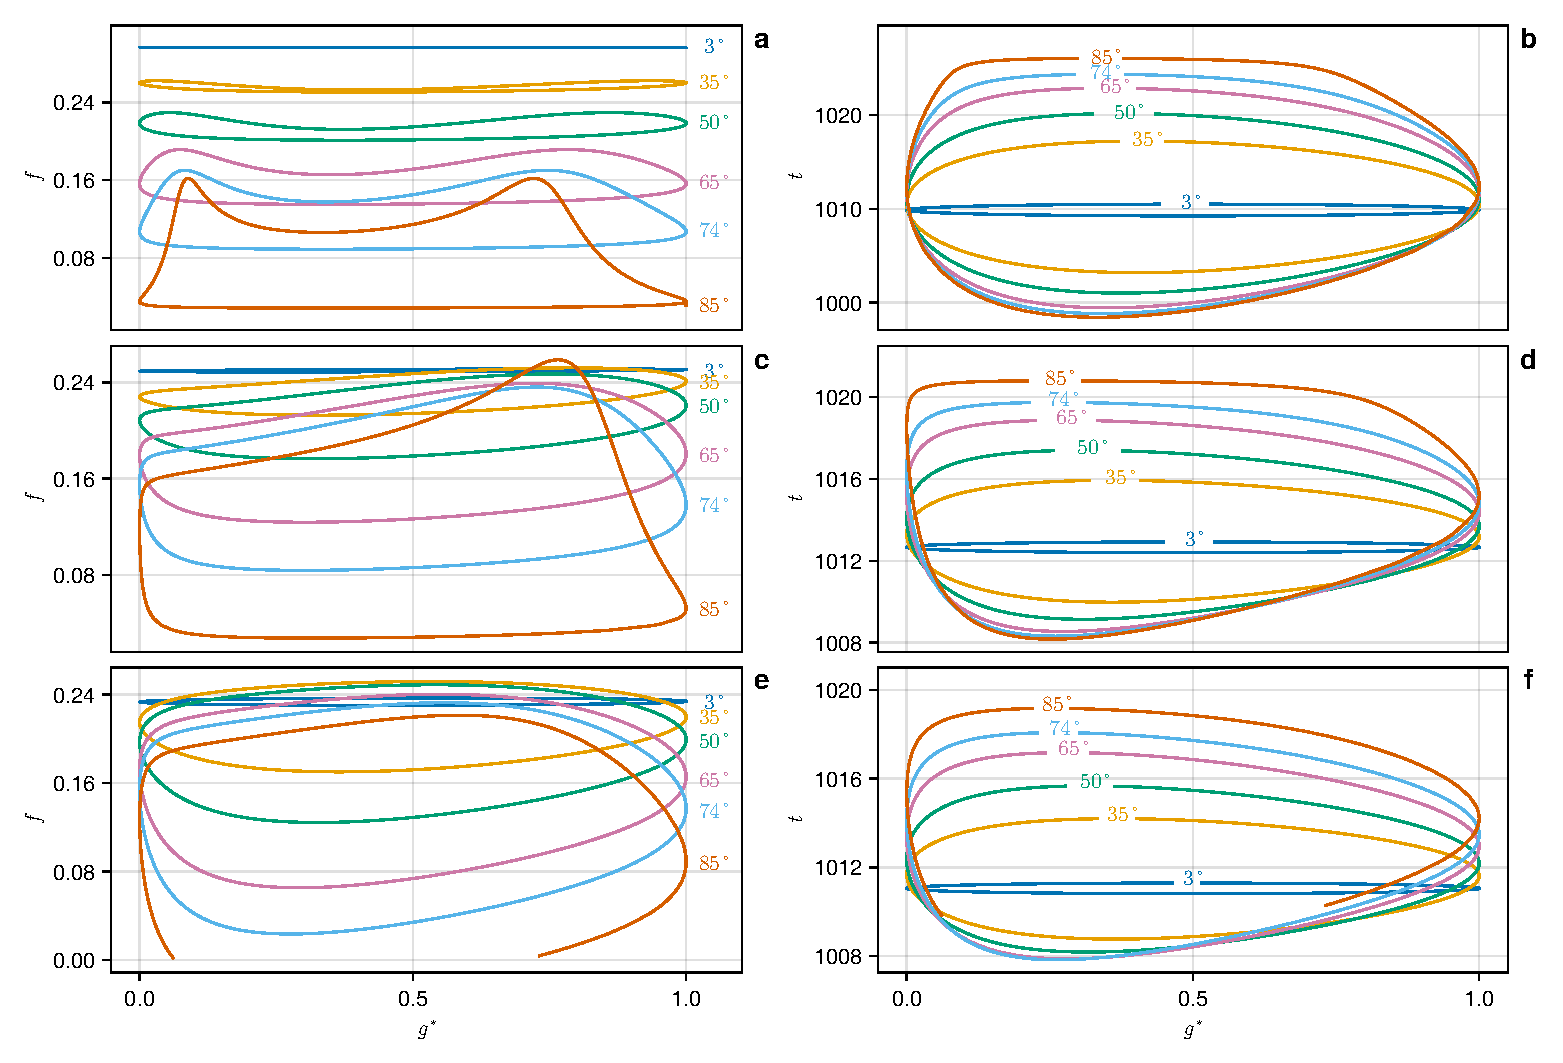
\includegraphics[width=0.99\linewidth]{figures/transfer-functions.plots.pdf}
    \caption{Transfer functions $f$ and timing $t$ for fixed $r_\text{em}$ for different observer inclinations $\theta_\text{obs}$ and $r_\text{obs} = 10^3 \rg$. Panels a) and b) Schwarzschild spacetime with equatorial thin disc and $r_\text{em} = 11\, \rg$. Panels c) and d) Maximally spinning Kerr spacetime $a=0.998$ with equatorial thin disc and $r_\text{em} = 4 \, \rg$ (see also \citealp{bambi_testing_2017}, their Figure 1). Panel e) and f) Maximally spinning Kerr spacetime $a=0.998$, with SSD $\dot{M} / \dot{M}_\text{Edd} = 0.3$ and $r_\text{em} = 4\, \rg$, showing obscuration at steep inclination.}
    \label{fig:transfer-functions}
\end{figure*}

\subsection{Integrating transfer functions}
\label{sec:transfer-function-integration}

Integrating $\d F(E)$ to calculate line-profiles is described in detail in \cite{dauser_broad_2010}, including the Green's function formalism that adds additional flexibility in the definition of $I_\text{em}$. The transfer functions are split into the aforementioned upper and lower branches at extremal $g^\ast$, and each branch is integrated separately, with the total summed in the final result. We extend the transfer function integration to include the geodesic coordinate time, integrating $f$ as

% \begin{strip}
% \rule[-1ex]{\columnwidth}{0.7pt}\rule[-1ex]{0.7pt}{1.5ex}
% \vbox{\vspace{2em}}
\begin{align}
    \label{eq:transfer-integration}
    F(E, t) &=
    \pi
    \int_0^\infty \d t^\prime \delta(t - t^\prime)
    \int_{r_\text{in}}^{r_\text{out}} \d r_\text{em}\,r_\text{em} \nonumber \\
    &\ \int_0^1 \d g^\ast\, \delta(E - gE_\text{line})\, g^2 I_\text{em}\left(\frac{E}{g}, t^\prime\right) \frac{f(r_\text{em}, g^\ast)}{\sqrt{g^\ast (1 - g^\ast)}},
\end{align}
% \vbox{\vspace{2em}}
% \hfill\rule[1ex]{0.7pt}{1.5ex}\rule[2.3ex]{\columnwidth}{0.7pt}
% \end{strip}
\noindent and $g = g( r_\text{em}, g^\ast, t')$ implicitly. The Dirac delta functions are selecting the $E$ and $t$ bin respectively. This allows us to construct high resolution lag transfer functions of \cite{reynolds_x-ray_1999} with little additional computational time (see Section \ref{sec:lag-transfer-functions}). 

The integrand for each branch remains in practice singular at $g^\ast \rightarrow (0, 1)$, and therefore the integration is performed over $g^\ast \in [h, 1 - h]$. Outside of this domain, the limits of the integrand can be taken to approximate the edges of the bin, as in \cite{dauser_broad_2010},
\begin{equation}
   F_\text{edge}(E,t) \propto 2\left( \sqrt{E_\text{max}} - \sqrt{E_\text{min}} \right).
\end{equation}
The constant of proportionality is determined from evaluating the integrand at $h$ or $1 - h$ respectively.

We use $h = 2 \times 10^{-6}$, and evaluate the integral over $\d g^\ast$ using a 7$^\text{th}$ order Gauss-Kronrod quadrature scheme, which avoids evaluating the integral directly at $h$ and $1 - h$ \citep{}. Finer grids for $r_\text{em}$ and $g^\ast$ are constructed to help with numerical accuracy and stability, with the finer bins subsequently rebinned into the desired output grid\footnote{The grid in $r$ should be irregularly spaced, e.g. $\sim 1 / r$, whereas the grid in $g$ should be linear. This reflects that the majority of the variation in $f$ occurs at small $r$.}.

The method for numerically integrating the time-dependent transfer functions is as follows: the limits of the integral are chosen $(r_\text{in}, r_\text{out})$, and limits of the output space similarly $(E_\text{min}, E_\text{max})$, $(t_\text{min}, t_\text{max})$. Any evaluation of \eqref{eq:transfer-integration} that is outside of the energy and time limits is discarded.  The integration over $\d r_\text{em}$ is simply performed using a trapezoidal scheme, as it is sufficient in both accuracy and performance with the finer bins. 

The $\d g^\ast$ quadrature scheme evaluates $F(E)$ for each branch over a small output bin in $g$, such that $t$ is determined by evaluating $t(g^\ast)$ at the limits of the bin, also for each branch. These approximations mandate that the integration is performed over a fine $g$ grid. In full:
\begin{enumerate}
    \item Interpolate the values of the transfer function, $f$, $t$, and $g_\text{min}$, and $g_\text{max}$, for the current radius $r_i$.
    \item Calculate the trapezoidal integration weight for the radial coordinate $\omega_i = \Delta r_i r_i$. Any other quantities that only depend on $r_\text{em}$ may similarly be factored into this weight, e.g. if $I_\text{em} = I_\text{em}(r_\text{em})$.
    \item For each bin in the fine $g$ grid, integrate $f$ over this bin. Record $t_\text{min} = t(g_\text{min})$ and $t_\text{max} = t(g_\text{max})$. Note that depending on the interpolation scheme, if $f$ is a function of $g$ instead of $g^\ast$, a $g / (g_\text{max} - g_\text{min})$ change-of-variable factor must be included in the integrand.
    \item Add $\omega_i F_i(E, t)$ to the bin corresponding to $E = gE_\text{line}$, and $t(g^\ast)$ for each branch. If either $\Delta E$ or $\Delta t$ straddles an output bin, the flux must be weighted appropriately and divided into those bins.
\end{enumerate}

By formulating the integration with the time component, we can use the same transfer function table to compute both line-profiles and reverberation lags efficiently, with arbitrary intensity functions $I_\text{em}$. We note that extensions to $I_\text{em}$ that require, for example, the photon emission angle on the disc, are trivial to include.

These transfer function integration methods may be checked for consistency against slower but simpler direct binning of the image plane via Eq. \eqref{eq:infinitesimal-flux} and Eq. \eqref{eq:liouville-theorem}.

\subsection{Covariant radiative transfer}

The intensity of a given geodesic is an observable that can be either calculated coincident with the geodesic trajectory, or retraced once the trajectory is determined.

The covariant formulation of the radiative transfer equation calculates the emissions and extinction in aframe co-moving with the geodesic \citep{fuerst_radiation_2004,younsi_general_2012}. The generalized form of the differential equation with respect to the affine parameter $\lambda$ is
\begin{equation}
    \label{eq:covariant-radiative-transfer}
    \frac{\d \mathcal{I}}{\d \lambda} = \left. \frac{\d s}{\d \lambda} \right\rvert_\lambda \left( -\alpha_\nu \mathcal{I} + \frac{j_\nu}{\nu^3} \right),
\end{equation}
where $\mathcal{I}$ is the invariant intensity, $s$ is the proper length traversed by the geodesic, and $\alpha_\nu$ and $j_\nu$ are the frequency $\nu$ dependent absorption and emissivity coefficients respectively, as measured in the local frame. The frequency $\nu$ is related to the observed frequency via the redshift
\begin{equation}
    g = \frac{\nu_\text{obs}}{\nu},
\end{equation}
In general, both coefficients $\alpha_nu$ and $j_\nu$ are also functions of the position $x^\mu$. 

The $\d s / \d \lambda$ derivative term is calculated by projecting the geodesic momentum $v_\mu$ onto the velocity $u^\mu$ of the medium, using the projection tensor
\begin{equation}
    \mathrm{P}^{\mu\nu} := g^{\mu\nu} + u^\mu u^\nu.
\end{equation}
The path length derivative is 
\begin{align}
    \left. \frac{\d s}{\d \lambda} \right\rvert_\lambda
    &= - \left. \left\lVert \mathrm{P}^{\mu\nu} v_\mu\right\rVert\, \right\rvert_\lambda,\\
    &= - \left. \sqrt{v_\mu v^\mu + \left(v_\mu u^\mu\right)^2 \left(2 + u^\mu u_\mu\right)} \, \right\rvert_\lambda,
\end{align}
such that for the particular case of null geodesics through a time-like medium
\begin{equation}
    \left. \frac{\d s}{\d \lambda} \right\rvert_\lambda = - \left. v_\mu u^\mu \right\rvert_\lambda.
\end{equation}

The covariant intensity $\mathcal{I}$ is related to the observed intensity $I_\nu = \mathcal{I} \nu^3$, derived using Liouville's theorem \citep{todo}. The intensity is therefore calculated by selecting $\nu_\text{obs} = E$ at the observer, and integrating \eqref{eq:covariant-radiative-transfer} along a given geodesic. 


%%% DESCRIPTION OF THE CODE %%%%%%%%%%%%%%%%%%%%%%
\section{Description of the code}

\Gradus is implemented in the Julia programming language \citep{Bezanson_Julia_A_fresh_2017}. We use the DifferentialEquations.jl ODE solving library and ForwardDiff.jl for forward-mode automatic differentiation \citep{RevelsLubinPapamarkou2016}. The code is available via the \texttt{Pkg} Julia package manger in a registry maintained by members of the University of Bristol astrophysics group\footnote{\url{https://github.com/astro-group-bristol/AstroRegistry/}}. There are also rudimentary bindings to a wide variety of languages, including Python via \texttt{pip} \citep{}.

\Gradus aims to have a single expressive high-level API for a variety of GRRT problems, with sensible defaults and optional fine-grained control. The code is accompanied by website documentation\footnote{\url{https://astro-group-bristol.github.io/Gradus.jl/}}, with short tutorials and examples designed to provide a feature-rich overview whilst simultaneously demonstrating how to construct custom simulations and how to integrate \Gradus in user models. We encourage readers who are interesting in learning up-to-date information about the code and our methods to consult the documentation, as the documentation strives to be the most accurate description of the code as it is maintained. The documentation details all algorithm specific choices and implementations, and is built as part of our continuous integration (CI). The source code is written to be read by contributors and users alike to invite extension, to be explicit about our methods, and their benefits and limitations.

\Gradus is extensively tested with a suite of unit and end-to-end tests. The tests are constructed both by comparing numerical algorithms to specific analytic counterparts, and by saving snapshots of results in the literature to compare against. The development cycle of \Gradus is thereby expedited, allowing changes to the codebase to be made with the confidence that no previous result will be broken.

In our discussion of the numerical methods, we note the current default ODE integration algorithm is Tsitouras Runge-Kutta 5/4. \Gradus vendors additional ODE solvers and numerical algorithms from the Julia SciML ecosystem, with both adaptive and fixed time steps, that may provide performance or accuracy improvements for specific problems.

\Gradus maintains a catalogue of predefined metrics, including the Kerr spacetime, Morris-Thorne wormhole, Johannsen-Psaltis metric, the Einstein-Maxwell Dilaton-Axion metric \todo{citations for these}, and the Kerr-Newman metric, complete with the ability to specify the electromagnetic potential vector, from which external accelerations $a^\mu$ in \eqref{eq:geodesic_equation} are calculated. \Gradus also has limited support for 1st order specification of the geodesic ODE system, where such a system is known. This is implemented for the Kerr spacetime, and used primarily as a self-consistency check with the second-order implementation.

\subsection{Extensibility}

Our implementations of the numerical methods, as well as the actual methods themselves, are conceptually simple and consequently generalize well. The design of \Gradus prioritizes useability and extensibility, which comes at a small performance cost: our aim is not to implement the fastest, semi-analytic solutions to specific problems, but rather to have an optimal and interpretable codebase for exploring problems related to general relativity. The abstractions in \Gradus have been designed to allow users to implement and calculate observables of their models quickly. To this end, we also include a number of visualization and plotting recipes to provide some intuition for the problem space.

\Gradus is designed to allow simple one-line changes to propagate through the simulations. The requisite calculations for determining observables have been abstracted in such a way that the precise function calls are determined at compile-time. This design is possible with Julia's just-in-time compilation and multiple dispatch, and bring additional benefits: different number types may be used through the whole library, permitting arbitrary precision floating point operations, symbolic evaluation through Symbolics.jl \citep{symbolics_julia}, or the propagation of AD gradient information through an entire simulation. Consequently, our code can calculate derivatives of any physical product with respect to the input parameters, and is therefore optimal for use directly in model fitting.

The shim we have implemented between our ODE problems and DifferentialEquations.jl allows additional quantities to be integrated along with the geodesic equation, as described in Section \ref{sec:computing-observables}. The abstraction permits users of \Gradus to easily specify new ODE components to be traced, if their model requires them. Many types in \Gradus are also composable, allowing complex simulations and calculations to be pieced together from simpler, testable components. Analytic accretion geometry may also be simply specified, and mesh geometry in common file formats may be readily imported.

Our transfer function integration routines permit arbitrary kernels, allowing any quantity integrated over the image plane to be efficiently pre-computed and calculated via transfer functions. Where additional information about the geodesics is needed, our extension to include the timing component serves as an example of the methods we have developed to permit this.

\subsection{Performance}
\label{sec:performance}

Our code makes use of Julia's heterogeneity and concurrency to run in multi-threaded and distributed environments, with GPU-offloading via DiffEqGPU.jl \citep{utkarsh2023automated}, and the various supported backends including CUDA and Metal \citep{besard2018juliagpu}. We have developed custom threading contexts that minimize allocated memory when tracing large numbers of geodesics.


\todo{a little talk about the threading strategies etc.}

\todo{GPU vs CPU and when one is one better than the other
Performance vs e.g. Bambi's NK and other work}

\subsection{Simulation products}

\todo{What we can export, and how they can be exported / used in e.g. XSPEC}

%%% TEST PROBLEMS %%%%%%%%%%%%%%%%%%%%%%%%%%%%%%%%
\section{Test problems}

\todo{explain why we compare those integrators}

\subsection{Integration accuracy and stability}

Since our method for integration does not use the constants of motion directly, the stability of the integrator may be gauged by sampling invariant quantities along the trajectory. In Figure \ref{fig:dot-stability} is shown the value the invariant of $v_\mu v^\mu$ for a geodesic that spirals into a maximally spinning black hole. The magnitude of the invariant is shown for a sample of integration algorithms, along with the solving time for the geodesic. Note this solving time includes the time to initialize the integrator, calculate the full trajectory (with interpolants), and package the solution structure. When tracing multiple geodesics, much of the initialization time may be avoided by reusing allocated memory -- see Section \ref{sec:performance}.

\begin{figure}
	\centering
	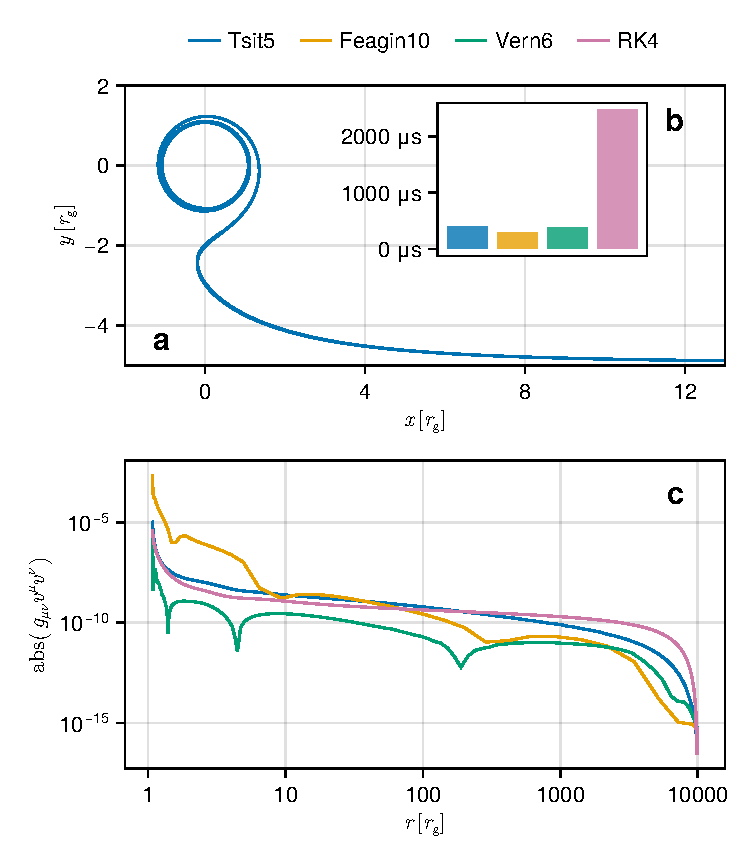
\includegraphics[width=0.95\linewidth]{figures/stability.conservation.pdf}
	\caption{\todo{caption + better choice of integrators to compare}}
	\label{fig:dot-stability}
\end{figure}

To test accuracy, we compare our numerical results with analytic values. The angular deflection is the difference in $x^\phi$ of a geodesic traveling from positive to negative infinity, that is
\begin{equation}
	\delta x^\phi :=
		x^\phi_{+\infty} - x^\phi_{-\infty} 
		- \pi,
\end{equation}
where the $-\pi$ is to account for radial change in the coordinate system between start and endpoint as the geodesic passes the origin \todo{is this right??}. Semi-analytic solutions for the deflection angle in the Kerr spacetime have been calculated for equatorial geodesics in \cite{iyer_lights_2009}, using elliptic integrals to find the coordinate differences. We follow their notation and denote the analytic deflection angle $\hat{\alpha}$, and present a compact summary of their calculations in Appendix \ref{appendix:deflection-angle}. 

Figure \ref{fig:deflection-angle} shows the deflection angle as a function of impact parameter $\alpha$ calculated using our code, along with the analytic deflection, and a measure of the error for different integration algorithms. Note the asymptotic behaviour of the error as $\lvert \alpha \rvert$ increases -- we account for this as related to the approximate observer at infinity in ray-tracing methods, catalyzed by the geometry of our observer introducing a small error at any finite $x^r$ when calculating the impact parameters relative to an $x^r = \infty$ observer. As can be expected, the error increases if $x^r_\text{start}$ is decreased.

\begin{figure}
	\centering
	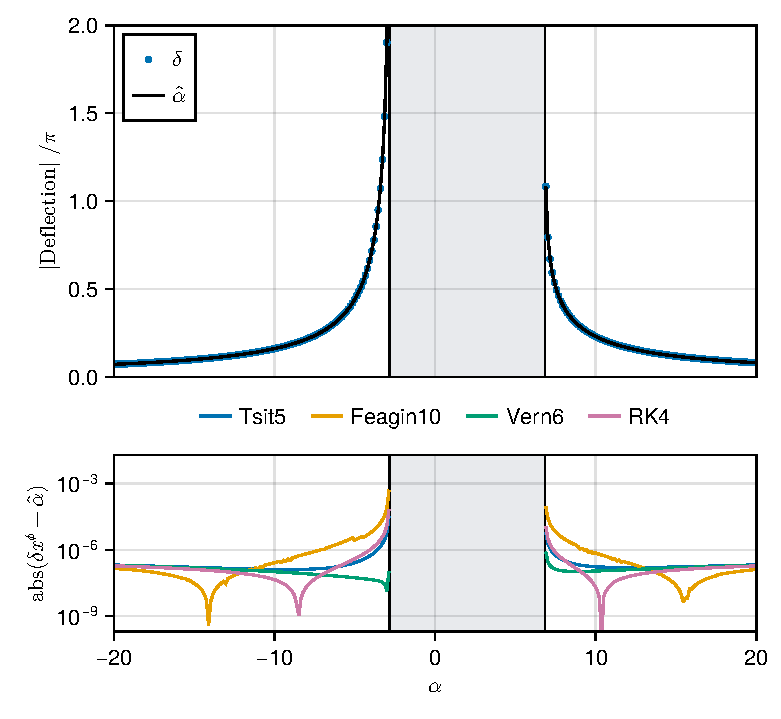
\includegraphics[width=0.94\linewidth]{figures/deflection.iyer-hansen.pdf}
	\caption{Deflection angle in the Kerr spacetime ($M = 1$, $a = 0.998$) for geodesics in the equatorial plane over a range of impact parameters $\alpha$. Upper panel: numerical deflection $\delta x^r$ calculated with  $x^r_\text{start} = 2 \times 10^8 \, \rg$, absolute and relative tolerances set to $10^{-14}$, and effective infinity $4 \times 10^8\, \rg$, shown with the numerical solutions for $\hat{\alpha}$. Lower panel: the absolute relative error between the numeric and analytic deflection angles for different integration algorithms.}
	\label{fig:deflection-angle}
\end{figure}


\todo{Energy conservation, deflection problem, shadow, tests for naked-singularities}


\subsection{Emissivity curves}

We calculate a number of emissivity profiles that have been published in the literature as a test of the numerical methods in Section \ref{sec:emissivity-profiles}. In Figure \ref{fig:emissivity-profiles} are shown the emissivity profiles for the lamp post corona at different heights, including the time difference due to the Shapiro delay. Our results are consistent with other authors \citep{wilkins_understanding_2012,dauser_irradiation_2013}.

\begin{figure}
	\centering
	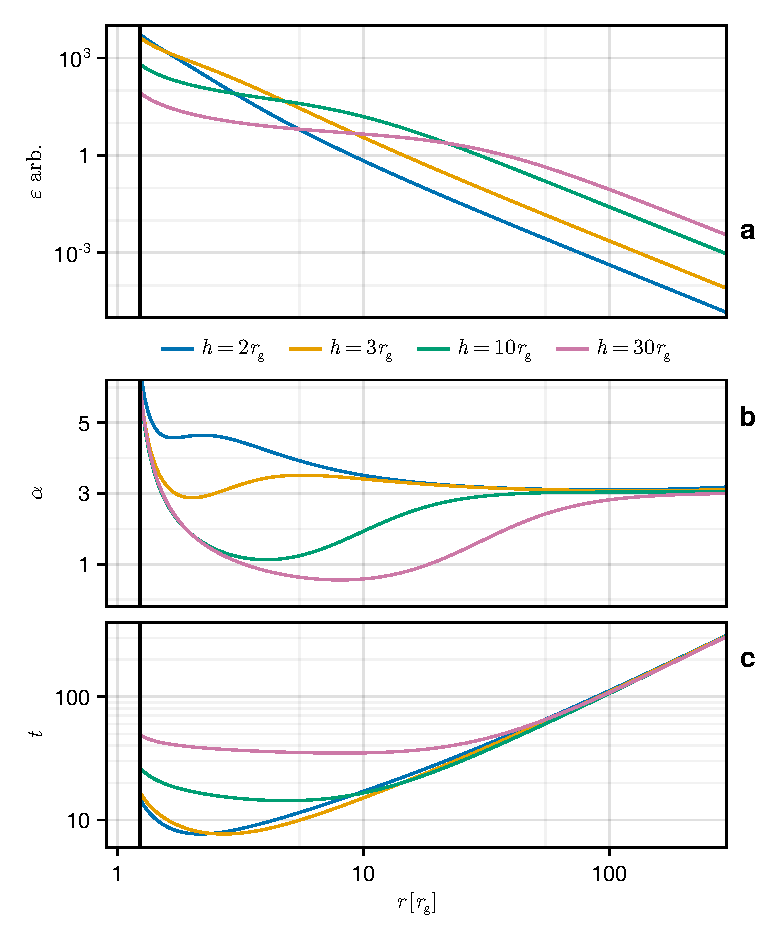
\includegraphics[width=0.99\linewidth]{figures/emissivity.point-source.pdf}
	\caption{\todo{caption}}
	\label{fig:emissivity-profiles}
\end{figure}

\todo{Wilkins and Fabian with lamp post and moving corona, gonzalez 2017}

\subsection{Line profiles}

Transfer functions are integrated as described in Section \ref{sec:transfer-function-integration}, neglecting the timing components. Figure \ref{fig:relline-comparison} compares the line profiles computed using the transfer functions of \Gradus and the \relline model of \cite{dauser_broad_2010}\footnote{We compare against the \relline v2.3 with table v0.5a distributed in the Relxill package \url{http://www.sternwarte.uni-erlangen.de/~dauser/research/relxill/}. These are the latest versions at time of writing.}. We see good agreement to within $\sim 1\%$ accuracy, with all features collocated.

\begin{figure}
	\centering
	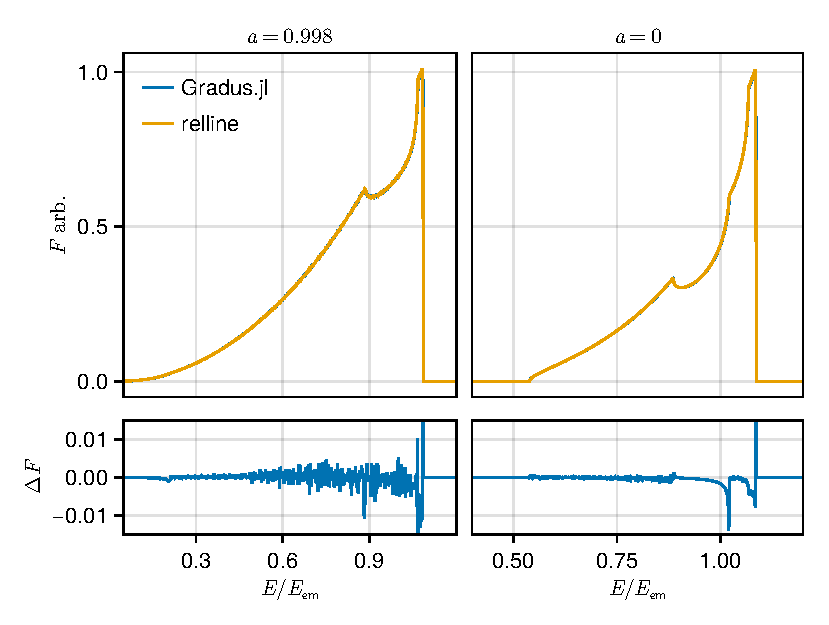
\includegraphics[width=0.99\linewidth]{figures/lineprofiles.comparison.pdf}
	\caption{Comparison of line profiles calculated by integrating transfer functions with emissivity $I_\text{em} = \varepsilon(r_\text{em}) = r_\text{em}^{-3}$ using \Gradus and \relline. The transfer functions are calculated for an observer at $r_\text{obs} = 1000\rg$ and $\theta_\text{obs} = 40^\circ$, and integrated between $r_\text{in} = \risco$ and $r_\text{out} = 50 \rg$. Left panel is the the maximally spinning Kerr spacetime, whereas the right panel is the Schwarzschild spacetime.}
	\label{fig:relline-comparison}
\end{figure}

Our code permits a consistency check by binning geodesics on the image plane, with the appropriate weighting. This method may also be used to compute line profiles for accretion geometry that does not lend itself to the transfer function parameterization. In Figure \ref{fig:line-profile-ssd}, we compute a number of line profiles for the SSD, using both the binning and transfer integration approach. \todo{finish this section}

\begin{figure}
	\centering
	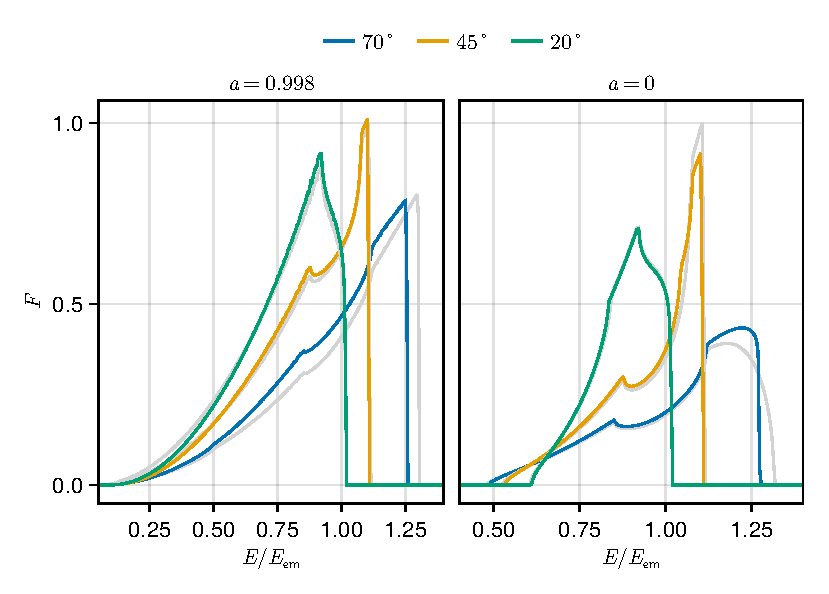
\includegraphics[width=0.99\linewidth]{figures/lineprofiles.ssd.pdf}
	\caption{Line profiles for the SSD with $\dot{M} / \dot{M}_\text{Edd} = 0.3$ for different observer inclinations $\theta_\text{obs}$ and emissivity $I_\text{em} = \varepsilon(r_\text{em}) = r_\text{em}^{-3}$. The transfer functions are calculated as in Figure \ref{fig:relline-comparison}, and integrated over the same limits. The light-grey lines correspond to the geometric thin disc ($\dot{M} / \dot{M}_\text{Edd} = 0$), and differ only for steep inclinations due to obscuration of inner $r_\text{em}$. Left panel is the the maximally spinning Kerr spacetime, whereas the right panel is the Schwarzschild spacetime.}
	\label{fig:line-profile-ssd}
\end{figure}


\subsection{Reverberation lags}
\label{sec:lag-transfer-functions}

\citep{reynolds_x-ray_1999,wilkins_origin_2013,cackett_modelling_2014}

\todo{Ingram's code? Jiachen's code}

\begin{figure}
	\centering
	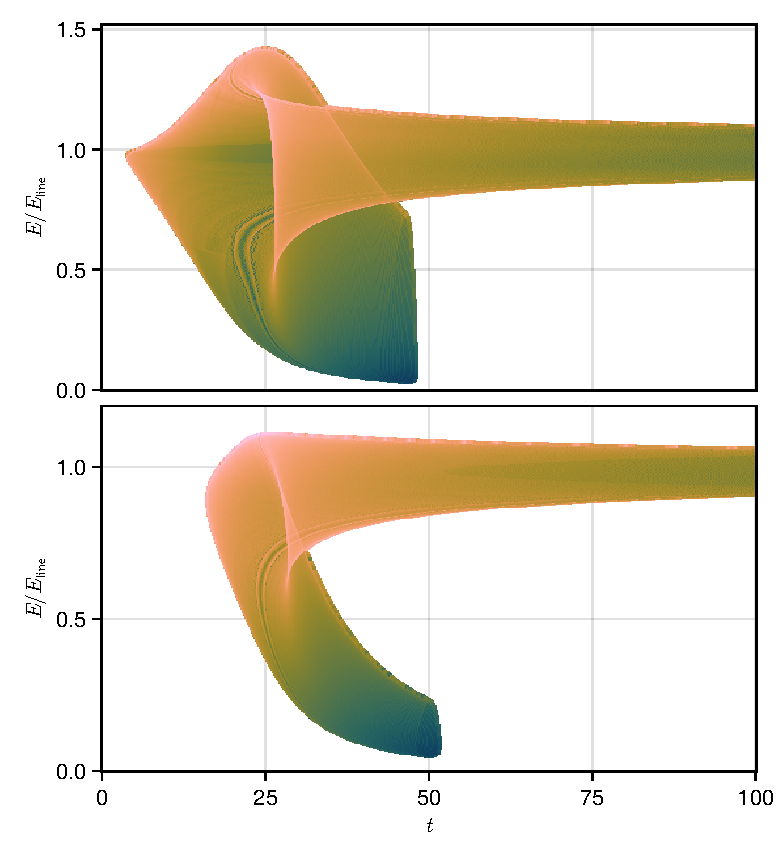
\includegraphics[width=0.97\linewidth]{figures/transfer-functions.2d.pdf}
	\caption{\todo{caption + slit is the gap between upper and lower branch contributions:: idea, interpolate when in h or 1-h}}
	\label{fig:lag-frequency-transfer-functions}
\end{figure}

\subsubsection{Lag-frequency spectra}

Summing the two dimensional transfer functions over the energy axis for a given energy range yields an impulse response $\psi(t)$, describing the time evolution of the observed flux. This impulse response depends on the properties of the illuminating corona, accretion disc, spacetime, and inclination of the observer. Examples for different lamp post heights over the full energy range are shown in the top panel of Figure \ref{fig:reverberation-thin}.

Following \cite{cackett_modelling_2014}, we define the \textit{response fraction} $R$ as the ratio of reflected to continuum flux. The impulse response in the Fourier domain is then the rescaled Fourier transform
\begin{equation}
	\mathscr{F}_\psi(f) := R \int_{0}^\infty \psi(t) \e^{-2\pi i f t} \d t.
\end{equation}
The phase difference between the reflected and continuum flux is 
\begin{equation}
	\phi(f) = \tan^{-1} \left( 
		\frac{\Im{\mathscr{F}_\psi}}{1 + \Re{\mathscr{F}_\psi}} 
	\right),
\end{equation}
where $\Im{\mathscr{F}_\psi}$ and $\Re{\mathscr{F}_\psi}$ are the imaginary and real components of $\mathscr{F}_\psi$ respectively. The imaginary component represents the lag contribution to the phase difference. Since the driving signal is present in both bands, it adds no lag contribution, but serves to dilute the phase difference and therefore the real component of the signal through the $+1$ in the denominator \citep{cackett_modelling_2014}. \todo{expand on this}

The time lag is defined as 
\begin{equation}
	\tau(f) := \frac{\phi}{2 \pi f},
\end{equation}
and relates the observed time lag to the Fourier frequency of the driving signal (lower panel of Figure \ref{fig:reverberation-thin}).

\begin{figure}
	\centering
	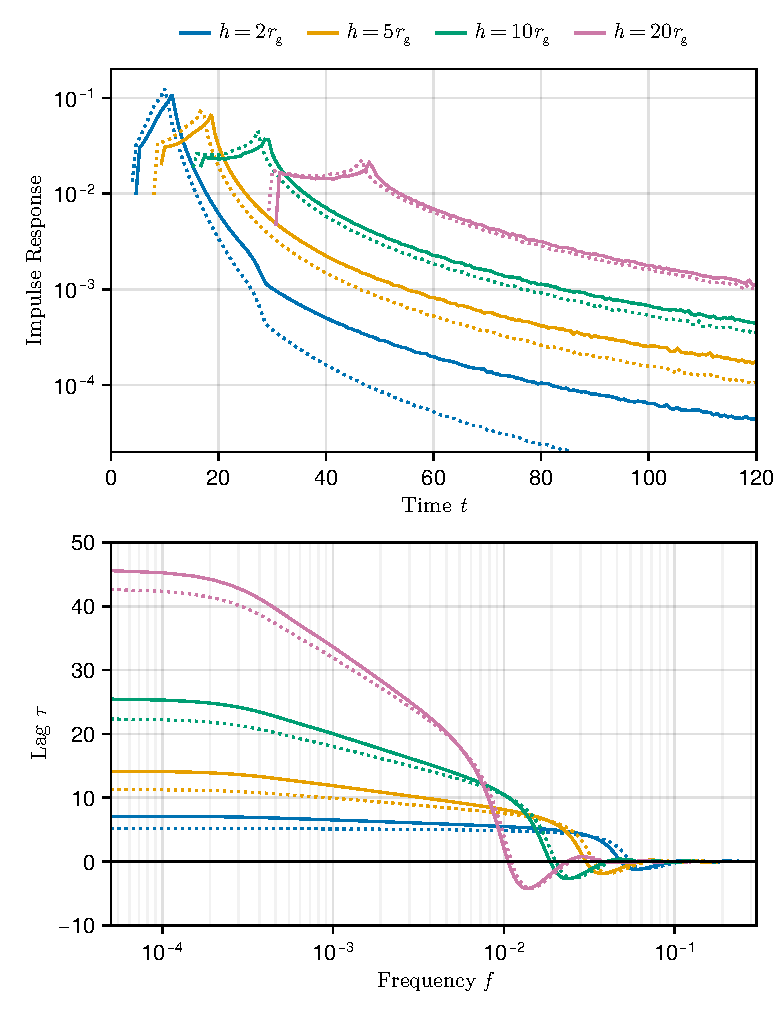
\includegraphics[width=0.98\linewidth]{figures/reverberation.thin-disc.pdf}
	\caption{\todo{TODO + move legend}}
	\label{fig:reverberation-thin}
\end{figure}

We note a slight disagreement with \cite{cackett_modelling_2014} in the $h = 10$ and $h=20$ case, due to a weak-field approximation after $100\, \rg$, which the authors employ for performance. At $\theta_\text{obs} = 45^\circ$ inclination, the time difference due to the weak-field approximation between the reflected and continuum band increases with $h$, resulting in their continuum component arriving \textit{early}. This results in a shift of the impulse response towards later $t$, and therefore a greater low frequency lag and a shift of the peak of the negative lag to lower $f$ (see Appendix \ref{appendix:continuum-time} for more detail).
\todo{maybe put this in an appendix and explain better with figures??}

\subsubsection{Lag-energy spectra}

\begin{figure}
	\centering
	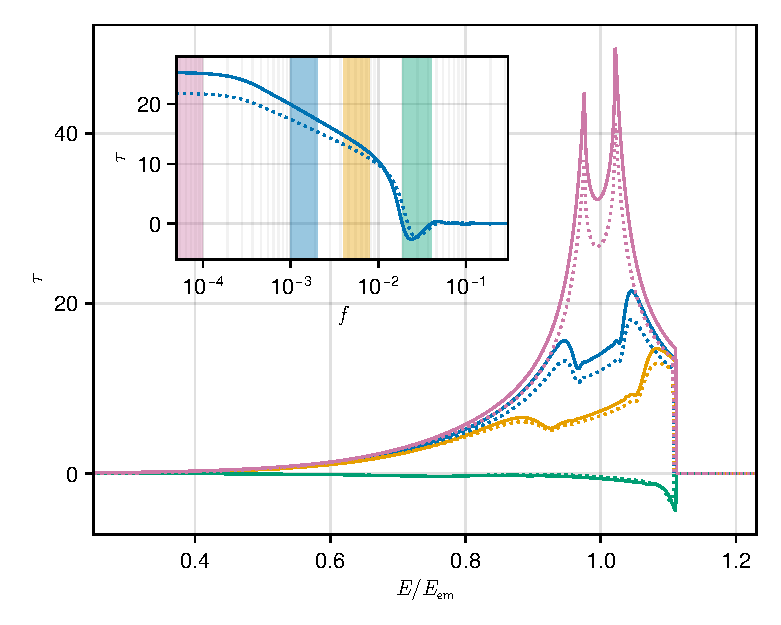
\includegraphics[width=0.98\linewidth]{figures/reverberation.lag-energy.pdf}
	\caption{\todo{TODO + move legend}}
	\label{fig:lag-energy}
\end{figure}


\subsection{Analytic radiative transfer model}

\cite{gold_verification_2020} specify an analytic model for testing radiative transfer codes (their Section 3.2, with results shown in their Figure 2 and 3). We have implemented their model and traced the radiative transfer problems with \Gradus, shown in Figure \ref{fig:gold-test-problems}. We find good agreement with the published results for all test problems.

\begin{figure*}
	\centering
	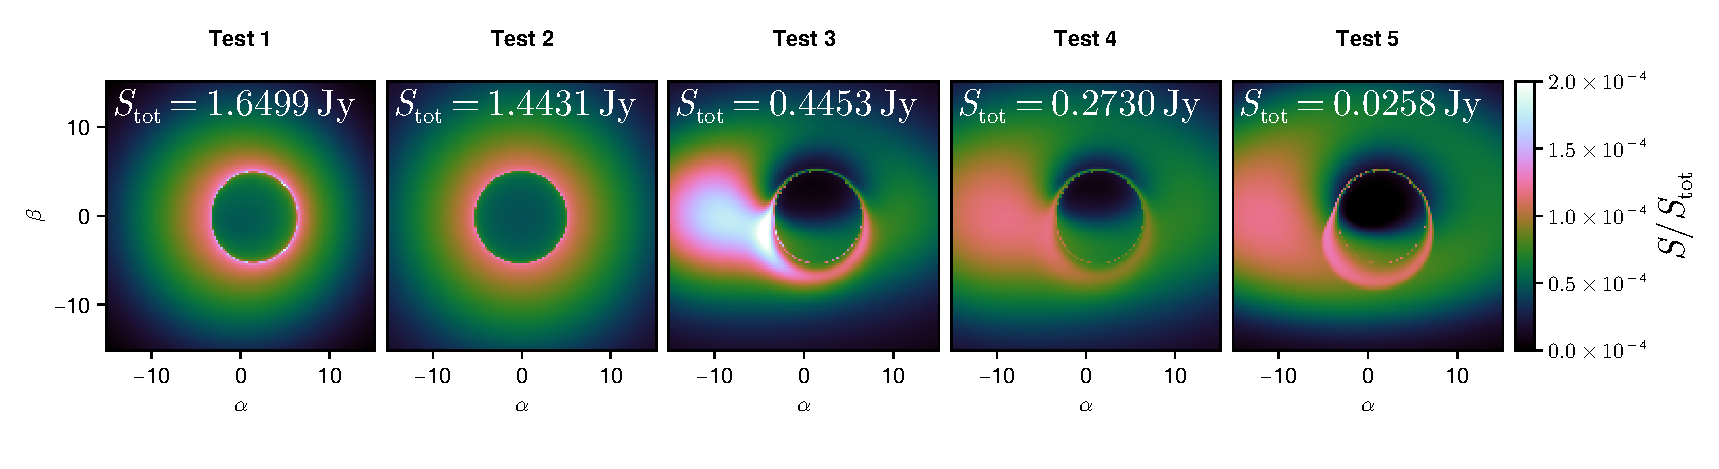
\includegraphics[width=0.99\linewidth]{figures/radiative-transfer.gold.pdf}
	\caption{Intensity images calculated with \Gradus of the radiative transfer analytic test models specified in \citet{gold_verification_2020} with resolution $128 \times 128$ pixels, and impact parameters ranging between $-15\, \rg$ and $15\, \rg$, and observer position $r_\text{obs} = 1000\, \rg$ and inclination $\theta_\text{obs} = 60^\circ$. The test cases correspond to the test parameters in their Table 1. The colouring is the intensity for the geodesic corresponding to that pixel normalized over the total intensity .}
	\label{fig:gold-test-problems}
\end{figure*}

\subsection{Other spacetimes}

Research into the appearance of compact singularities in modified gravity theories is often focused on the shadow of the singularity or the photon rings.

\cite{bambi_testing_2017,abdikamalov_testing_2020} have created a suite of codes \texttt{ABHModels}\footnote{\todo{add link}} for studying the iron line and reflection spectra from accreting black holes in the Johannsen metric. This metric is constructed by taking a higher order multipole expansion of the spherical harmonics of the metric \citep{johannsen_regular_2013}. Their codes are able to calculate lineprofiles and black-body disc spectra for the various deformation parameters of the Johannsen metric. Their code is however limited to a choice of a single deformation parameter, due to the method by which they construct their geodesic implementation. 

We compare the line profiles for the Johannsen metric in Figure \ref{fig:compare-johannsen}.

\todo{Bambi's various metrics and relline, self consistency between methods}
\todo{iron line profiles for Johannsen Psaltis}
\todo{geodesic motion of kerr newman}

\section{Applications}

\todo{working on spectral and timing models (Baker et al. in prep) for use in XSPEC and beyond}

\todo{working on propagating gradient information from models into spectral fitting pipelines}

\todo{including radiative transfer information in the transfer functions}

We are working on a optimized thick disc spectral and reverberation model for use in spectral fitting programs based on our thick disc transfer functions and time-dependant transfer function integration. 

\section{Conclusions}

We encourage the community to contact us with interesting problems that may be tackled using \Gradus as we are happy to assist with new applications of the code.

\todo{problems with the code are being patched, see github issues}

% Note future work, e.g., with regard to fitting, and using the code in other papers

\section*{Acknowledgements}
This work is supported by the UKRI AIMLAC CDT funded by grant EP/S023992/1.

We thank Jiachen Jiang, Cosimo Bambi and Askar Abdikamalov for sharing their software for comparisons. FB thanks Rosie for her expert debugging assistance, and Shaun for invaluable software discussions. All figures created using Makie.jl \citep{DanischKrumbiegel2021}, using the color scheme of \cite{wong_points_2011}.

%%%%%%%%%%%%%%%%%%%%%%%%%%%%%%%%%%%%%%%%%%%%%%%%%%
\section*{Data Availability}

No new data or analyses have been created for this work. The code to reproduce this paper and all figures therein is freely available under MIT license:
\url{https://github.com/fjebaker/gradus-paper}


% The inclusion of a Data Availability Statement is a requirement for articles published in MNRAS. Data Availability Statements provide a standardised format for readers to understand the availability of data underlying the research results described in the article. The statement may refer to original data generated in the course of the study or to third-party data analysed in the article. The statement should describe and provide means of access, where possible, by linking to the data or providing the required accession numbers for the relevant databases or DOIs.

%%%%%%%%%%%%%%%%%%%% REFERENCES %%%%%%%%%%%%%%%%%%

% The best way to enter references is to use BibTeX:

\bibliographystyle{mnras}
\bibliography{citations} % if your bibtex file is called example.bib


%%%%%%%%%%%%%%%%%%%%%%%%%%%%%%%%%%%%%%%%%%%%%%%%%%

%%%%%%%%%%%%%%%%% APPENDICES %%%%%%%%%%%%%%%%%%%%%

\appendix

\section{orthonormalization with Gram-Schmidt}
\label{appendix:gram-schmidt}

The theorem of Gram-Schmidt states that it is always possible to construct a set of orthonormal vectors in any inner-product space $\mathbb{R}^n$, and uses a projection-subtraction procedure as a proof \citep{schmidt_uber_1989}. Starting with $n$ linearly independent vectors $\vector{v}_n$, and denoting the projection of a vector $\vector{u}$ along the direction of $\vector{v}$ as
\begin{equation}
\mathrm{P}_{\vector{v}}\left(\vector{u}\right) := \frac{\vector{v} \cdot \vector{u}}{\vector{u} \cdot \vector{u}}\ \vector{u} = \frac{g_{\mu\nu} v^\mu u^\nu}{g_{\sigma\rho} u^\sigma u^\rho} \vector{u},
\end{equation}
allows expressing the Gram-Schmidt procedure as
\begin{align}
    \vector{k}_1 &= \vector{v}_1, \nonumber \\
    \vector{k}_2 &= \vector{v}_2 - \mathrm{P}_{\vector{k}_1}\left(\vector{v}_2 \right), \nonumber \\
    &\vdots \nonumber \\
    \vector{k}_n &= \vector{v}_n - \sum_{i = 1}^{n-1} \mathrm{P}_{\vector{k}_i} \left(\vector{v}_n \right).
\end{align}
Constructing meaningful orthonormal frames requires appropriate choice of the initial linearly independent vectors $\vector{v}$, in order to associate global directions with the tetrad. The locally non-rotating frame (LNRF), with angular velocity $\omega = -g_{t\phi} / g_{\phi\phi}$, has tangential frame velocity $v^\mu = A (1, 0, 0, \omega)$ where $A$ is some normalization. To construct the LNRF, a choice of initial vectors may therefore be
\begin{align}
    \vector{v}_1 &= \left(1, 0, 0, \omega \right) \mapsto \dtensor{\e}{(t)}{\mu}, \nonumber \\
    \vector{v}_2 &= \left(1, 0, 0, 1\right) \mapsto \dtensor{\e}{(\phi)}{\mu}, \nonumber \\
    \vector{v}_3 &= \left(1, 1, 0, 1\right) \mapsto \dtensor{\e}{(r)}{\mu}, \nonumber \\
    \vector{v}_4 &= \left(1, 1, 1, 1\right) \mapsto \dtensor{\e}{(\theta)}{\mu},
\end{align}
where we have denoted the corresponding tetrad vector generated by the orthonormalization procedure after the arrow.

Other sensible frames require different initial vectors, and care must be taken in implementing a method that correctly reorders the resulting tetrad vectors: for example, the zero angular momentum (ZAMO) frame for an on-axis coronal source with velocity $\dot{x}^\mu = (1, \d r / \d t, 0, 0)$ requires
\begin{align}
    \vector{v}_1 &= \left(1, \d r / \d t, 0, 0 \right) \mapsto \dtensor{\e}{(t)}{\mu}, \nonumber \\
    \vector{v}_2 &= \left(1, 1, 0, 0\right) \mapsto \dtensor{\e}{(r)}{\mu}, \nonumber \\
    \vector{v}_3 &= \left(1, 1, 1, 0\right) \mapsto \dtensor{\e}{(\theta)}{\mu}, \nonumber \\
    \vector{v}_4 &= \left(1, 1, 1, 1\right) \mapsto \dtensor{\e}{(\phi)}{\mu}.
\end{align}

Our implementation of the Gram-Schmidt procedure is accurate up to machine-level with the analytic tetrads for the LNRF in \cite{bardeen_rotating_1972}, their Equation (3.2), and for the moving source ZAMO frame in \cite{gonzalez_probing_2017}, their Equation (10).

\section{Keplerian orbits of static, axis-symmetric spacetimes with accelerated geodesics}
\label{appendix:circular-orbits}
% \section{Semi-analytic deflection angle for static, axis-symmetric spacetimes}
\label{appendix:deflection-angle}


\section{On the numerical errors in the choice of ODE integrator}
\label{appendix:solvers}

Efforts to compare GRRT codes inevitably face the same problem; that analytic (`true') results to compare to can only be constructed for contrived or simplified models. Instead, there is a tendency to attempt to compare geodesic calculations, often nearing machine precision, as a method of evaluating the accuracy of a given code. A particular fallacy is that calculating with arbitrary precision floating point numbers will in some sense convey a result that is closer to the `truth'. There is however inherent bias in this approach, as the choice of integrator for precisely the same configuration contributes an error that can be significant.

A recent paper showed the choice of ingoing and out-going Eddington-Finkelstein coordinates contributes certain errors in certain GRRT problems, in particular for geodesics close to the event horizon. The magnitude of these errors, however, is far smaller than the difference in choice of integrator.

Taking a different number of steps close to the event horizon alters the floating point error due to the non-commutativity of floting point operations.

\todo{\cite{Rackaukas} has investigated Runge-Kutta tableaus }

\todo{We conclude codes that agree to within $\sqrt{\varepsilon}$...}


\section{Caution against a weak field approximation}
\label{appendix:continuum-time}

A weak field approximation for general relativistic effects is sometimes used in the interest of computational performance. For example, a spherical radius $R$ outside of which relativistic effects are said to be negligible, such that a flat (Minkowski) spacetime metric is used for ray-tracing and other calculations. In \citet{cackett_modelling_2014}, $R = 100\, \rg$ is used when calculating lag-frequency and lag-energy spectra. However, this approximation introduces a slight error when calculating the light travel time of flux from the disc and continuum source, which has a surprisingly significant effect on the computed lag-frequency spectra.

Since \Gradus is metric agnostic, we implement a new spacetime that switches to the Minkwoski form beyond $R$ and recalculate the lag-frequency relations. Our implementation preserves constant of motions across the boundary when switching from one metric to another, though other weak-field approximations may not, introducing additional errors in the trajectories of geodesics that depend on the ODE integration algorithm used and the solver steps over the boundary.

% The use of this weak-field approximation reproduces the results of \citet{cackett_modelling_2014}, but differs from the lag-frequency curve presented in this paper. We offer the following explanation:

% In cases where the source height above the black hole is small, the systematic error from the weak field approximation between the reflected and continuum flux is approximately equal, and therefore is negligible when the difference in arrival time is calculated, as in
% \begin{equation}
%     \Delta t = \tilde{t}_\text{reflected} - \tilde{t}_\text{continuum} ,
% \end{equation}
% where the tilde denotes the inclusion of some $\delta t$ due to the weak field approximation $\tilde{t} = t_\text{true} - \delta t$. However, when the source height is of appreciable value, say $h > 10\rg$, then for an off axis observer the systematic error introduced by $\delta t$ is greater for the continuum emission than for the reflected component (see Figure \ref{fig:app:weak-field-approx}), resulting in the continuum flux arriving seemingly too early. Note that $\delta t$ is dependant on the observer's position, and decreases with increasing $r_\text{obs}$.

% Figure \ref{fig:app:continuum-time} illustrates the relationship between coronal source height and $\delta t$, calculated by using the weak field approximation at different $R$ and subtracting the equivalent `true' light travel time $t$ (equivalent to $R \rightarrow \infty$). Even at $h = 100$, the continuum flux from the corona is seen to arrive significantly early.

% \begin{figure}
% 	\centering
% 	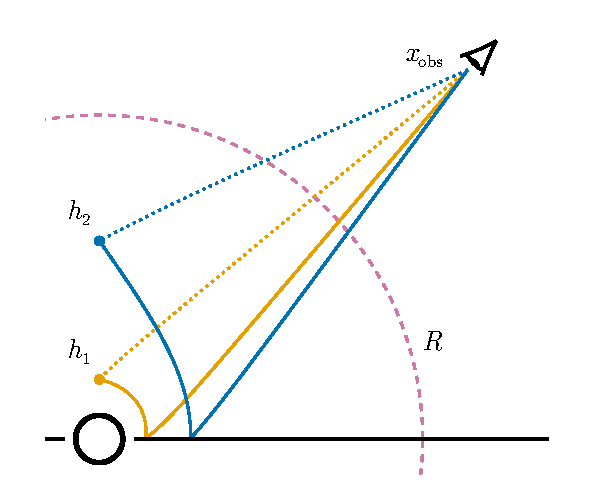
\includegraphics[width=0.80\linewidth]{figures/continuum-time.figure.pdf}
% 	\caption{\todo{TODO}}
% 	\label{fig:app:weak-field-approx}
% \end{figure}

% For the source heights of $h=10\, \rg$ and $h = 20 \rg$ and an observer inclination of $\theta_\text{obs} = 45^\circ$, the path length of the traject

% \todo{a heatmap showing $\delta t$ for different $h$ and observer distances?}

% \begin{figure}
% 	\centering
% 	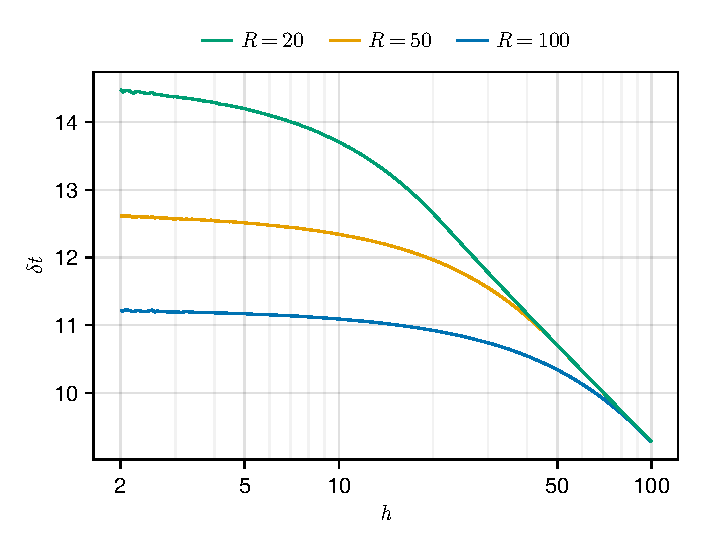
\includegraphics[width=0.98\linewidth]{figures/continuum-time.weak-field.pdf}
% 	\caption{\todo{TODO}}
% 	\label{fig:app:continuum-time}
% \end{figure}


% \section{Some extra material}

%%%%%%%%%%%%%%%%%%%%%%%%%%%%%%%%%%%%%%%%%%%%%%%%%%


% Don't change these lines
\bsp	% typesetting comment
\label{lastpage}
\end{document}

% End of mnras_template.tex
